%-----------------------------------------------------------------------------------------
% Autor dieser Vorlage:
% Stefan Macke (http://fachinformatiker-anwendungsentwicklung.net)
% Permalink zur Vorlage: http://fiae.link/LaTeXVorlageFIAE
% Lizenz: Creative Commons 4.0 Namensnennung - Weitergabe unter gleichen Bedingungen
% -----------------------------------------------------------------------------------------

\documentclass[
	ngerman,
	toc=listof, % Abbildungsverzeichnis sowie Tabellenverzeichnis in das Inhaltsverzeichnis aufnehmen
	toc=bibliography, % Literaturverzeichnis in das Inhaltsverzeichnis aufnehmen
	footnotes=multiple, % Trennen von direkt aufeinander folgenden Fußnoten
	parskip=half, % vertikalen Abstand zwischen Absätzen verwenden anstatt horizontale Einrückung von Folgeabsätzen
	numbers=noendperiod, % Den letzten Punkt nach einer Nummerierung entfernen (nach DIN 5008)
	13pt
]{scrartcl}
\pdfminorversion=5 % erlaubt das Einfügen von pdf-Dateien bis Version 1.7, ohne eine Fehlermeldung zu werfen (keine Garantie für fehlerfreies Einbetten!)
\usepackage[utf8]{inputenc} % muss als erstes eingebunden werden, da Meta/Packages ggfs. Sonderzeichen enthalten

% !TEX root = Ausarbeitung.tex

% Hinweis: der Titel muss zum Inhalt des Projekts passen und den zentralen Inhalt des Projekts deutlich herausstellen
\newcommand{\titel}{Software-Container und Software-Development}
\newcommand{\untertitel}{Bedeutung und Risiken von Software-Containern, sowie deren Einsatz in der Softwareentwicklung und das Zusammenspiel in Clustern}
\newcommand{\kompletterTitel}{\titel{} -- \untertitel}


\newcommand{\betriebLogo}{logo.png}


\newcommand{\betreff}{Praktische Arbeit zur vorbereitenden Blockveranstaltung}
 % Metadaten zu diesem Dokument (Autor usw.)
% !TEX root = ../Ausarbeitung.tex

% Anpassung an Landessprache ---------------------------------------------------
\usepackage{babel}

% Umlaute ----------------------------------------------------------------------
%   Umlaute/Sonderzeichen wie äüöß direkt im Quelltext verwenden (CodePage).
%   Erlaubt automatische Trennung von Worten mit Umlauten.
% ------------------------------------------------------------------------------
\usepackage[T1]{fontenc}
\usepackage{textcomp} % Euro-Zeichen etc.
% Schrift ----------------------------------------------------------------------
%\usepackage{lmodern} % bessere Fonts
\usepackage{relsize} % Schriftgröße relativ festlegen

% Tabellen ---------------------------------------------------------------------
\PassOptionsToPackage{table}{xcolor}
\usepackage{tabularx}
% für lange Tabellen
\usepackage{longtable}
\usepackage{array}
\usepackage{ragged2e}
\usepackage{lscape}
\newcolumntype{w}[1]{>{\raggedleft\hspace{0pt}}p{#1}} % Spaltendefinition rechtsbündig mit definierter Breite

% Grafiken ---------------------------------------------------------------------
\usepackage[dvips,final]{graphicx} % Einbinden von JPG-Grafiken ermöglichen
\usepackage{graphics} % keepaspectratio
\usepackage{float} % zum Umfließen von Bildern
\usepackage{wrapfig} % zum Umfließen von Bildern
\graphicspath{{Bilder/}} % hier liegen die Bilder des Dokuments


% Sonstiges --------------------------------------------------------------------
\usepackage[titles]{tocloft} % Inhaltsverzeichnis DIN 5008 gerecht einrücken
\usepackage{amsmath,amsfonts} % Befehle aus AMSTeX für mathematische Symbole
\usepackage{enumitem} % anpassbare Enumerates/Itemizes
\usepackage{xspace} % sorgt dafür, dass Leerzeichen hinter parameterlosen Makros nicht als Makroendezeichen interpretiert werden

\usepackage{makeidx} % für Index-Ausgabe mit \printindex
\usepackage[printonlyused]{acronym} % es werden nur benutzte Definitionen aufgelistet

\usepackage{datetime} % Angabe des Build-Datums auf dem Deckblatt

% Einfache Definition der Zeilenabstände und Seitenränder etc.
\usepackage{setspace}
\usepackage{geometry}

% Symbolverzeichnis
\usepackage[intoc]{nomencl}
\let\abbrev\nomenclature
\renewcommand{\nomname}{Abkürzungsverzeichnis}
\setlength{\nomlabelwidth}{.25\hsize}
\renewcommand{\nomlabel}[1]{#1 \dotfill}
\setlength{\nomitemsep}{-\parsep}

\usepackage{varioref} % Elegantere Verweise. „auf der nächsten Seite“
\usepackage{url} % URL verlinken, lange URLs umbrechen etc.

\usepackage{chngcntr} % fortlaufendes Durchnummerieren der Fußnoten
% \usepackage[perpage]{footmisc} % Alternative: Nummerierung der Fußnoten auf jeder Seite neu

\usepackage{ifthen} % bei der Definition eigener Befehle benötigt
\usepackage{todonotes} % definiert u.a. die Befehle \todo und \listoftodos
\usepackage[square]{natbib} % wichtig für korrekte Zitierweise
\usepackage{float}
% PDF-Optionen -----------------------------------------------------------------
\usepackage{pdfpages}
\pdfminorversion=5 % erlaubt das Einfügen von pdf-Dateien bis Version 1.7, ohne eine Fehlermeldung zu werfen (keine Garantie für fehlerfreies Einbetten!)
\usepackage[
    bookmarks,
    bookmarksnumbered,
    bookmarksopen=true,
    bookmarksopenlevel=1,
    colorlinks=true,
% diese Farbdefinitionen zeichnen Links im PDF farblich aus
    linkcolor=AOBlau, % einfache interne Verknüpfungen
    anchorcolor=AOBlau,% Ankertext
    citecolor=AOBlau, % Verweise auf Literaturverzeichniseinträge im Text
    filecolor=AOBlau, % Verknüpfungen, die lokale Dateien öffnen
    menucolor=AOBlau, % Acrobat-Menüpunkte
    urlcolor=AOBlau,
% diese Farbdefinitionen sollten für den Druck verwendet werden (alles schwarz)
    %linkcolor=black, % einfache interne Verknüpfungen
    %anchorcolor=black, % Ankertext
    %citecolor=black, % Verweise auf Literaturverzeichniseinträge im Text
    %filecolor=black, % Verknüpfungen, die lokale Dateien öffnen
    %menucolor=black, % Acrobat-Menüpunkte
    %urlcolor=black,
%
    %backref, % Quellen werden zurück auf ihre Zitate verlinkt
    pdftex,
    plainpages=false, % zur korrekten Erstellung der Bookmarks
    pdfpagelabels=true, % zur korrekten Erstellung der Bookmarks
    hypertexnames=false, % zur korrekten Erstellung der Bookmarks
    linktocpage % Seitenzahlen anstatt Text im Inhaltsverzeichnis verlinken
]{hyperref}
% Befehle, die Umlaute ausgeben, führen zu Fehlern, wenn sie hyperref als Optionen übergeben werden
\hypersetup{
    pdftitle={\titel -- \untertitel},
    pdfsubject={\titel -- \untertitel},
    pdfkeywords={\titel -- \untertitel},
}


% zum Einbinden von Programmcode -----------------------------------------------
\usepackage{listings}
\usepackage{xcolor}
\definecolor{hellgelb}{rgb}{1,1,0.9}
\definecolor{colKeys}{rgb}{0,0,1}
\definecolor{colIdentifier}{rgb}{0,0,0}
\definecolor{colComments}{rgb}{0,0.5,0}
\definecolor{colString}{rgb}{1,0,0}
\lstset{
    float=hbp,
	basicstyle=\ttfamily\footnotesize,
    identifierstyle=\color{colIdentifier},
    keywordstyle=\color{colKeys},
    stringstyle=\color{colString},
    commentstyle=\color{colComments},
    backgroundcolor=\color{white},
    columns=flexible,
    tabsize=2,
    frame=single,
    extendedchars=true,
    showspaces=false,
    showstringspaces=false,
    numbers=left,
    numberstyle=\tiny,
    breaklines=true,
    breakautoindent=true,
	captionpos=b,
}
\lstdefinelanguage{cs}{
    language=[Sharp]C,
    frame=lrb
	sensitive=false,
	morecomment=[l]{//},
	morecomment=[s]{/*}{*/},
	morestring=[b]",
	morekeywords={
		abstract,event,new,struct,as,explicit,null,switch
		base,extern,object,this,bool,false,operator,throw,
		break,finally,out,true,byte,fixed,override,try,
		case,float,params,typeof,catch,for,private,uint,
		char,foreach,protected,ulong,checked,goto,public,unchecked,
		class,if,readonly,unsafe,const,implicit,ref,ushort,
		continue,in,return,using,decimal,int,sbyte,virtual,
		default,interface,sealed,volatile,delegate,internal,short,void,
		do,is,sizeof,while,double,lock,stackalloc,
		else,long,static,enum,namespace,string},
}
\lstdefinelanguage{natural}{
	sensitive=false,
	morecomment=[l]{/*},
	morestring=[b]",
	morestring=[b]',
	alsodigit={-,*},
	morekeywords={
		DEFINE,DATA,LOCAL,END-DEFINE,WRITE,CALLNAT,PARAMETER,USING,
		IF,NOT,END-IF,ON,*ERROR-NR,ERROR,END-ERROR,ESCAPE,ROUTINE,
		PERFORM,SUBROUTINE,END-SUBROUTINE,CONST,END-FOR,END,FOR,RESIZE,
		ARRAY,TO,BY,VALUE,RESET,COMPRESS,INTO,EQ},
}
\lstdefinelanguage{php}{
	sensitive=false,
	morecomment=[l]{/*},
	morestring=[b]",
	morestring=[b]',
	alsodigit={-,*},
	morekeywords={
		abstract,and,array,as,break,case,catch,cfunction,class,clone,const,
		continue,declare,default,do,else,elseif,enddeclare,endfor,endforeach,
		endif,endswitch,endwhile,extends,final,for,foreach,function,global,
		goto,if,implements,interface,instanceof,namespace,new,old_function,or,
		private,protected,public,static,switch,throw,try,use,var,while,xor
		die,echo,empty,exit,eval,include,include_once,isset,list,require,
		require_once,return,print,unset},
}
 % verwendete Packages
% !TEX root = ../Ausarbeitung.tex

% Seitenränder -----------------------------------------------------------------
\setlength{\topskip}{\ht\strutbox} % behebt Warnung von geometry
\geometry{a4paper,left=30mm,right=30mm,top=30mm,bottom=35mm}

\usepackage[
	automark, % Kapitelangaben in Kopfzeile automatisch erstellen
	headsepline, % Trennlinie unter Kopfzeile
	ilines % Trennlinie linksbündig ausrichten
]{scrpage2}

% Kopf- und Fußzeilen ----------------------------------------------------------
\pagestyle{scrheadings}
% chapterpagestyle gibt es nicht in scrartcl
%\renewcommand{\chapterpagestyle}{scrheadings}
\clearscrheadfoot

% Kopfzeile
\renewcommand{\headfont}{\normalfont} % Schriftform der Kopfzeile
\ihead{\textsc{\titel}\\[0.5ex] \textit{\headmark}}
\chead{}
\ohead{\includegraphics[scale=0.1]{\betriebLogo}}
\setlength{\headheight}{15mm} % Höhe der Kopfzeile
%\setheadwidth[0pt]{textwithmarginpar} % Kopfzeile über den Text hinaus verbreitern (falls Logo den Text überdeckt)

% Fußzeile
\ifoot{\today}
\cfoot{}
\ofoot{\pagemark}

% Überschriften nach DIN 5008 in einer Fluchtlinie
% ------------------------------------------------------------------------------

% Abstand zwischen Nummerierung und Überschrift definieren
% > Schön wäre hier die dynamische Berechnung des Abstandes in Abhängigkeit
% > der Verschachtelungstiefe des Inhaltsverzeichnisses
\newcommand{\headingSpace}{1.5cm}

% Abschnittsüberschriften im selben Stil wie beim Inhaltsverzeichnis einrücken
\renewcommand*{\othersectionlevelsformat}[3]{
  \makebox[\headingSpace][l]{#3\autodot}
}

% Für die Einrückung wird das Paket tocloft benötigt
%\cftsetindents{chapter}{0.0cm}{\headingSpace}
\cftsetindents{section}{0.0cm}{\headingSpace}
\cftsetindents{subsection}{0.0cm}{\headingSpace}
\cftsetindents{subsubsection}{0.0cm}{\headingSpace}
\cftsetindents{figure}{0.0cm}{\headingSpace}
\cftsetindents{table}{0.0cm}{\headingSpace}


% Allgemeines
% ------------------------------------------------------------------------------

\onehalfspacing % Zeilenabstand 1,5 Zeilen
\frenchspacing % erzeugt ein wenig mehr Platz hinter einem Punkt

% Schusterjungen und Hurenkinder vermeiden
\clubpenalty = 10000
\widowpenalty = 10000
\displaywidowpenalty = 10000

% Quellcode-Ausgabe formatieren
%\lstset{numbers=left, numberstyle=\tiny, numbersep=5pt, breaklines=true}
\lstset{emph={square}, emphstyle=\color{red}, emph={[2]root,base}, emphstyle={[2]\color{blue}}}

\counterwithout{footnote}{section} % Fußnoten fortlaufend durchnummerieren
\setcounter{tocdepth}{\subsubsectionlevel} % im Inhaltsverzeichnis werden die Kapitel bis zum Level der subsubsection übernommen
\setcounter{secnumdepth}{\subsubsectionlevel} % Kapitel bis zum Level der subsubsection werden nummeriert

% Aufzählungen anpassen
\renewcommand{\labelenumi}{\arabic{enumi}.}
\renewcommand{\labelenumii}{\arabic{enumi}.\arabic{enumii}.}
\renewcommand{\labelenumiii}{\arabic{enumi}.\arabic{enumii}.\arabic{enumiii}}

% Tabellenfärbung:
\definecolor{heading}{rgb}{0.64,0.78,0.86}
\definecolor{odd}{rgb}{0.9,0.9,0.9}

% Schriftart
\usepackage[sfdefault, scale=1, light]{roboto}  % Roboto als Schrifart
\usepackage[T1]{fontenc}
\usepackage{newtxsf}
 % Definitionen zum Aussehen der Seiten
% !TEX root = ../Projektdokumentation.tex

% Abkürzungen, ggfs. mit korrektem Leerraum
\newcommand{\bs}{$\backslash$\xspace}
\newcommand{\bspw}{bspw.\xspace}
\newcommand{\bzw}{bzw.\xspace}
\newcommand{\ca}{ca.\xspace}
\newcommand{\dahe}{\mbox{d.\,h.}\xspace}
\newcommand{\etc}{etc.\xspace}
\newcommand{\eur}[1]{\mbox{#1\,\texteuro}\xspace}
\newcommand{\evtl}{evtl.\xspace}
\newcommand{\ggfs}{ggfs.\xspace}
\newcommand{\Ggfs}{Ggfs.\xspace}
\newcommand{\gqq}[1]{\glqq{}#1\grqq{}}
\newcommand{\inkl}{inkl.\xspace}
\newcommand{\insb}{insb.\xspace}
\newcommand{\ua}{\mbox{u.\,a.}\xspace}
\newcommand{\usw}{usw.\xspace}
\newcommand{\Vgl}{Vgl.\xspace}
\newcommand{\zB}{\mbox{z.\,B.}\xspace}

% Befehle für häufig anfallende Aufgaben
\newcommand{\Abbildung}[1]{\autoref{fig:#1}}
\newcommand{\Anhang}[1]{\appendixname{}~\ref{#1}: \nameref{#1} \vpageref{#1}}
\newcommand{\Abschnitt}[1]{\autoref{sec:#1}: \nameref{sec:#1}}
\newcommand{\includegraphicsKeepAspectRatio}[2]{\includegraphics[width=#2\textwidth,height=#2\textheight,keepaspectratio]{#1}}
\newcommand{\Zitat}[2][\empty]{\ifthenelse{\equal{#1}{\empty}}{\citep{#2}}{\citep[#1]{#2}}}
\newcommand{\Autor}[1]{\textsc{#1}} % zum Ausgeben von Autoren
\newcommand{\itemd}[2]{\item{\textbf{#1}}\\{#2}} % erzeugt ein Listenelement mit fetter Überschrift
\newcommand{\Grafik}[4] % Parameter: caption, label, breite, file (in /Bilder)
{\begin{figure}[H]
        \begin{center}
            \includegraphics[width=#3\textwidth]{../Bilder/#4}
        \end{center}
        \caption{#1}
        \label{fig:#2}
\end{figure}}
\newcommand{\Grafikraw}[2] % Parameter: breite, file (in /Bilder)
{\begin{figure}[H]
        \begin{center}
            \includegraphics[width=#1\textwidth]{#2}
        \end{center}
\end{figure}}

% fügt Tabellen aus einer TEX-Datei ein
\newcommand{\tabelle}[3] % Parameter: caption, label, file
{\begin{table}[htbp]
\centering
\singlespacing
\input{Tabellen/#3}
\caption{#1}
\label{#2}
\end{table}}

\newcommand{\tabelleAnhang}[1] % Parameter: file
{\begin{center}
\singlespacing
\input{Tabellen/#1}
\end{center}}

% einfaches Wechseln der Schrift, z.B.: \changefont{cmss}{sbc}{n}
\newcommand{\changefont}[3]{\fontfamily{#1} \fontseries{#2} \fontshape{#3} \selectfont}

% Verwendung analog zu \includegraphics
\newlength{\myx} % Variable zum Speichern der Bildbreite
\newlength{\myy} % Variable zum Speichern der Bildhöhe
\newcommand\includegraphicstotab[2][\relax]{%
% Abspeichern der Bildabmessungen
\settowidth{\myx}{\includegraphics[{#1}]{#2}}%
\settoheight{\myy}{\includegraphics[{#1}]{#2}}%
% das eigentliche Einfügen
\parbox[c][1.1\myy][c]{\myx}{%
\includegraphics[{#1}]{#2}}%
}

\definecolor{AOBlau}{rgb}{0, 0.28, 0.56}

% verschiedene Befehle um Wörter semantisch auszuzeichnen ----------------------
\newcommand{\Index}[2][\empty]{\ifthenelse{\equal{#1}{\empty}}{\index{#2}#2}{\index{#1}#2}}
\newcommand{\Fachbegriff}[2][\empty]{\ifthenelse{\equal{#1}{\empty}}{\textit{\Index{#2}}}{\textit{\Index[#1]{#2}}}}
\newcommand{\NeuerBegriff}[2][\empty]{\ifthenelse{\equal{#1}{\empty}}{\textbf{\Index{#2}}}{\textbf{\Index[#1]{#2}}}}

\newcommand{\Ausgabe}[1]{\texttt{#1}}
\newcommand{\Eingabe}[1]{\texttt{#1}}
\newcommand{\Code}[1]{\texttt{#1}}
\newcommand{\Datei}[1]{\texttt{#1}}

\newcommand{\Assembly}[1]{\textsf{#1}}
\newcommand{\Klasse}[1]{\textsf{#1}}
\newcommand{\Methode}[1]{\textsf{#1}}
\newcommand{\Attribut}[1]{\textsf{#1}}

\newcommand{\Datentyp}[1]{\textsf{#1}}
\newcommand{\XMLElement}[1]{\textsf{#1}}
\newcommand{\Webservice}[1]{\textsf{#1}}

\newcommand{\Refactoring}[1]{\Fachbegriff{#1}}
\newcommand{\CodeSmell}[1]{\Fachbegriff{#1}}
\newcommand{\Metrik}[1]{\Fachbegriff{#1}}
\newcommand{\DesignPattern}[1]{\Fachbegriff{#1}}

\newcommand{\quelle}[1]{\footnote{\scriptsize Quelle: \url{#1}}}
\newcommand{\quellefoot}[2]{\footnotetext[#1]{\tiny Quelle: \url{#2}}}
\newcommand{\refAbbildung}[1]{(\hyperref[#1]{Abbildung \ref*{#1}})}
\newcommand{\UK}{$\text{U}_{\text{K}0}$}

\newcommand{\Abbildung}[1]{\autoref{fig:#1}}
\newcommand{\Anhang}[1]{\appendixname{}~\ref{#1}: \nameref{#1} \vpageref{#1}}
\newcommand{\Abschnitt}[1]{\autoref{sec:#1}: \nameref{sec:#1}}
 % eigene allgemeine Befehle, die z.B. die Arbeit mit LaTeX erleichtern
% !TEX root = ../Projektdokumentation.tex

% Abkürzungen, ggfs. mit korrektem Leerraum
\newcommand{\bs}{$\backslash$\xspace}
\newcommand{\bspw}{bspw.\xspace}
\newcommand{\bzw}{bzw.\xspace}
\newcommand{\ca}{ca.\xspace}
\newcommand{\dahe}{\mbox{d.\,h.}\xspace}
\newcommand{\etc}{etc.\xspace}
\newcommand{\eur}[1]{\mbox{#1\,\texteuro}\xspace}
\newcommand{\evtl}{evtl.\xspace}
\newcommand{\ggfs}{ggfs.\xspace}
\newcommand{\Ggfs}{Ggfs.\xspace}
\newcommand{\gqq}[1]{\glqq{}#1\grqq{}}
\newcommand{\inkl}{inkl.\xspace}
\newcommand{\insb}{insb.\xspace}
\newcommand{\ua}{\mbox{u.\,a.}\xspace}
\newcommand{\usw}{usw.\xspace}
\newcommand{\Vgl}{Vgl.\xspace}
\newcommand{\zB}{\mbox{z.\,B.}\xspace}

% Befehle für häufig anfallende Aufgaben
\newcommand{\Abbildung}[1]{\autoref{fig:#1}}
\newcommand{\Anhang}[1]{\appendixname{}~\ref{#1}: \nameref{#1} \vpageref{#1}}
\newcommand{\Abschnitt}[1]{\autoref{sec:#1}: \nameref{sec:#1}}
\newcommand{\includegraphicsKeepAspectRatio}[2]{\includegraphics[width=#2\textwidth,height=#2\textheight,keepaspectratio]{#1}}
\newcommand{\Zitat}[2][\empty]{\ifthenelse{\equal{#1}{\empty}}{\citep{#2}}{\citep[#1]{#2}}}
\newcommand{\Autor}[1]{\textsc{#1}} % zum Ausgeben von Autoren
\newcommand{\itemd}[2]{\item{\textbf{#1}}\\{#2}} % erzeugt ein Listenelement mit fetter Überschrift
\newcommand{\Grafik}[4] % Parameter: caption, label, breite, file (in /Bilder)
{\begin{figure}[H]
        \begin{center}
            \includegraphics[width=#3\textwidth]{../Bilder/#4}
        \end{center}
        \caption{#1}
        \label{fig:#2}
\end{figure}}
\newcommand{\Grafikraw}[2] % Parameter: breite, file (in /Bilder)
{\begin{figure}[H]
        \begin{center}
            \includegraphics[width=#1\textwidth]{#2}
        \end{center}
\end{figure}}

% fügt Tabellen aus einer TEX-Datei ein
\newcommand{\tabelle}[3] % Parameter: caption, label, file
{\begin{table}[htbp]
\centering
\singlespacing
\input{Tabellen/#3}
\caption{#1}
\label{#2}
\end{table}}

\newcommand{\tabelleAnhang}[1] % Parameter: file
{\begin{center}
\singlespacing
\input{Tabellen/#1}
\end{center}}

% einfaches Wechseln der Schrift, z.B.: \changefont{cmss}{sbc}{n}
\newcommand{\changefont}[3]{\fontfamily{#1} \fontseries{#2} \fontshape{#3} \selectfont}

% Verwendung analog zu \includegraphics
\newlength{\myx} % Variable zum Speichern der Bildbreite
\newlength{\myy} % Variable zum Speichern der Bildhöhe
\newcommand\includegraphicstotab[2][\relax]{%
% Abspeichern der Bildabmessungen
\settowidth{\myx}{\includegraphics[{#1}]{#2}}%
\settoheight{\myy}{\includegraphics[{#1}]{#2}}%
% das eigentliche Einfügen
\parbox[c][1.1\myy][c]{\myx}{%
\includegraphics[{#1}]{#2}}%
}

\definecolor{AOBlau}{rgb}{0, 0.28, 0.56}

% verschiedene Befehle um Wörter semantisch auszuzeichnen ----------------------
\newcommand{\Index}[2][\empty]{\ifthenelse{\equal{#1}{\empty}}{\index{#2}#2}{\index{#1}#2}}
\newcommand{\Fachbegriff}[2][\empty]{\ifthenelse{\equal{#1}{\empty}}{\textit{\Index{#2}}}{\textit{\Index[#1]{#2}}}}
\newcommand{\NeuerBegriff}[2][\empty]{\ifthenelse{\equal{#1}{\empty}}{\textbf{\Index{#2}}}{\textbf{\Index[#1]{#2}}}}

\newcommand{\Ausgabe}[1]{\texttt{#1}}
\newcommand{\Eingabe}[1]{\texttt{#1}}
\newcommand{\Code}[1]{\texttt{#1}}
\newcommand{\Datei}[1]{\texttt{#1}}

\newcommand{\Assembly}[1]{\textsf{#1}}
\newcommand{\Klasse}[1]{\textsf{#1}}
\newcommand{\Methode}[1]{\textsf{#1}}
\newcommand{\Attribut}[1]{\textsf{#1}}

\newcommand{\Datentyp}[1]{\textsf{#1}}
\newcommand{\XMLElement}[1]{\textsf{#1}}
\newcommand{\Webservice}[1]{\textsf{#1}}

\newcommand{\Refactoring}[1]{\Fachbegriff{#1}}
\newcommand{\CodeSmell}[1]{\Fachbegriff{#1}}
\newcommand{\Metrik}[1]{\Fachbegriff{#1}}
\newcommand{\DesignPattern}[1]{\Fachbegriff{#1}}

\newcommand{\quelle}[1]{\footnote{\scriptsize Quelle: \url{#1}}}
\newcommand{\quellefoot}[2]{\footnotetext[#1]{\tiny Quelle: \url{#2}}}
\newcommand{\refAbbildung}[1]{(\hyperref[#1]{Abbildung \ref*{#1}})}
\newcommand{\UK}{$\text{U}_{\text{K}0}$}

\newcommand{\Abbildung}[1]{\autoref{fig:#1}}
\newcommand{\Anhang}[1]{\appendixname{}~\ref{#1}: \nameref{#1} \vpageref{#1}}
\newcommand{\Abschnitt}[1]{\autoref{sec:#1}: \nameref{sec:#1}}
 % eigene projektspezifische Befehle, z.B. Abkürzungen usw.

\begin{document}


\phantomsection
\thispagestyle{plain}
\pdfbookmark[1]{Deckblatt}{deckblatt}
%!TEX root = Projektdokumentation.tex
\begin{titlepage}

\begin{center}

\includegraphics[scale=0.25]{logo.png}\\[5ex]


\large{\betreff}\\[3.5ex]

\LARGE{\textbf{\titel}}\\[1.5ex]
\large{\untertitel}\\[3.5ex]

\normalsize

\begin{tabular}{c c}

\end{tabular}

\textbf{\Large{Autoren:}}\\
    \begin{tabular}{c c}
        \\
        Maximilian Rieger & Florian Lubitz\\
        Technische Informatik & Technische Informatik\\
        85581 & 85900\\
        \\
        Thomas Schöller & Marc Bitzer\\
        Technische Informatik & Technische Informatik\\
        87113 & 87117\\
        \\
        \multicolumn{2}{c}{Jonas Acker}\\
        \multicolumn{2}{c}{Technische Informatik}\\
        \multicolumn{2}{c}{85583}\\
    \end{tabular}
\\[3ex]

\end{center}

\end{titlepage}
\cleardoublepage

% Preface --------------------------------------------------------------------
\phantomsection
\pagenumbering{gobble}
%\pagenumbering{arabic}
\setcounter{tocdepth}{2}
\pdfbookmark[1]{Inhaltsverzeichnis}{inhalt}
\tableofcontents
\cleardoublepage


\pagenumbering{arabic}
% Inhalt ---------------------------------------------------------------------
% !TEX root = Projektdokumentation.tex
% !TEX root = ../Ausarbeitung.tex
\section{Einleitung}
\label{sec:Einleitung}
Bis kurz vor der Jahrtausendwende führte die Virtualisierung von Servern ein Schattendasein und jeder Service wurde auf einem dedizierten Server zur Verfügung gestellt.
Dabei war es keine Seltenheit, dass Server sehr gering ausgelastet waren, da der laufende Service nicht die gesamte Leistung der Hardware benötigte und der Ausfall eines nicht redundanten Servers einen Totalausfall eines Services bedeutete.
Eine Beispielhafte dedizierte Serverkonstellation stellt Grafik \ref{fig:HW1} dar.
\begin{figure}[H]
	\begin{center}
		
\includegraphics[width=1\textwidth]{vm1.png}
	\end{center}
	\caption[Serverauslastung ohne Virtualisierung]{Serverauslastung ohne Virtualisierung \footnotemark}
	\label{fig:HW1}
\end{figure}
\quellefoot{https://www.redhat.com/cms/managed-files/server-usage-500x131.png}
\newpage
Um diese und weitere Probleme zu lösen, gewann die Virtualisierung von Servern zum Anfang des neuen Jahrtausends immer mehr an Bedeutung und ist heutzutage ein fester Bestandteil vieler großer Unternehmen.
Dabei werden auf einem physikalischen System mehrere Dienste zusammengefasst, die sonst nur einen Bruchteil der Leistung benötigen würden.
Dadurch kommen noch andere Vorteile wie z.B. das Erstellen von Snapshots und das dynamische Verschieben der virtuellen Maschinen zum Tragen.
Grafik \ref{fig:HW2} zeigt die Auslastung der virtualisieren Server.
\begin{figure}[H]
	\begin{center}
		
\includegraphics[width=1\textwidth]{vm2.png}
	\end{center}
	\caption[Serverauslastung mit Virtualisierung]{Serverauslastung mit Virtualisierung \footnotemark}
	\label{fig:HW2}
\end{figure}
\quellefoot{https://www.redhat.com/cms/managed-files/server-usage-for-virtualization-500x131.png}
\newpage
Doch auch die Virtualisierung von Servern birgt noch Probleme, die einer Lösung bedürfen.
So entsteht durch das Betriebssystem der virtuellen Maschinen ein deutlicher Overhead, da diese zur Laufzeit etliche Services benötigen.
Außerdem beanspruchen die virtualisierten Betriebssysteme deutlich mehr Hardwareressourcen und die Startzeit ist relativ lang.
Somit war die IT-Branche nicht in der Lage, wozu die Transportbranche längst in der Lage war: Güter in Container zu verpacken und diese Container aufgrund des standardisierten Formats auf den verschiedensten Verkehrswegen zu transportieren.
\begin{figure}[H]
	\begin{center}
		
\includegraphics[width=1\textwidth]{Schiffscontainer.jpg}
	\end{center}
	\caption[Container]{Container \footnotemark}
	\label{fig:schffscontainer}
\end{figure}
\quellefoot{http://tricon-terminal.de/uploads/pics/_MG_8745_06.jpg}
Um diese Lösung in die IT zu portieren, wurden auch für diese Problemstellung Container (in dem Fall für Software) entwickelt.
Software-Container setzen wie die Schiffscontainer an dem Punkt Portabilität an.
Es soll nicht für jeden Service ein zusätzliches Betriebssystem virtualisiert werden, sondern der Container soll nur das zusätzlich beinhalten, was er für den Service benötigt und trotzdem isoliert von den anderen Container auf der Hardware laufen.
Außerdem soll es wie bei den virtuellen Maschinen möglich sein, dynamisch Ressourcen zuzuweisen.\cite{12005068320161201,redhat} 
\newpage
Die Grafik \ref{fig:VergleichContainerVM} verdeutlicht nochmals den eingesparten Overhead bei Containern verglichen mit virtuellen Maschinen.
\begin{figure}[H]
	\begin{center}
		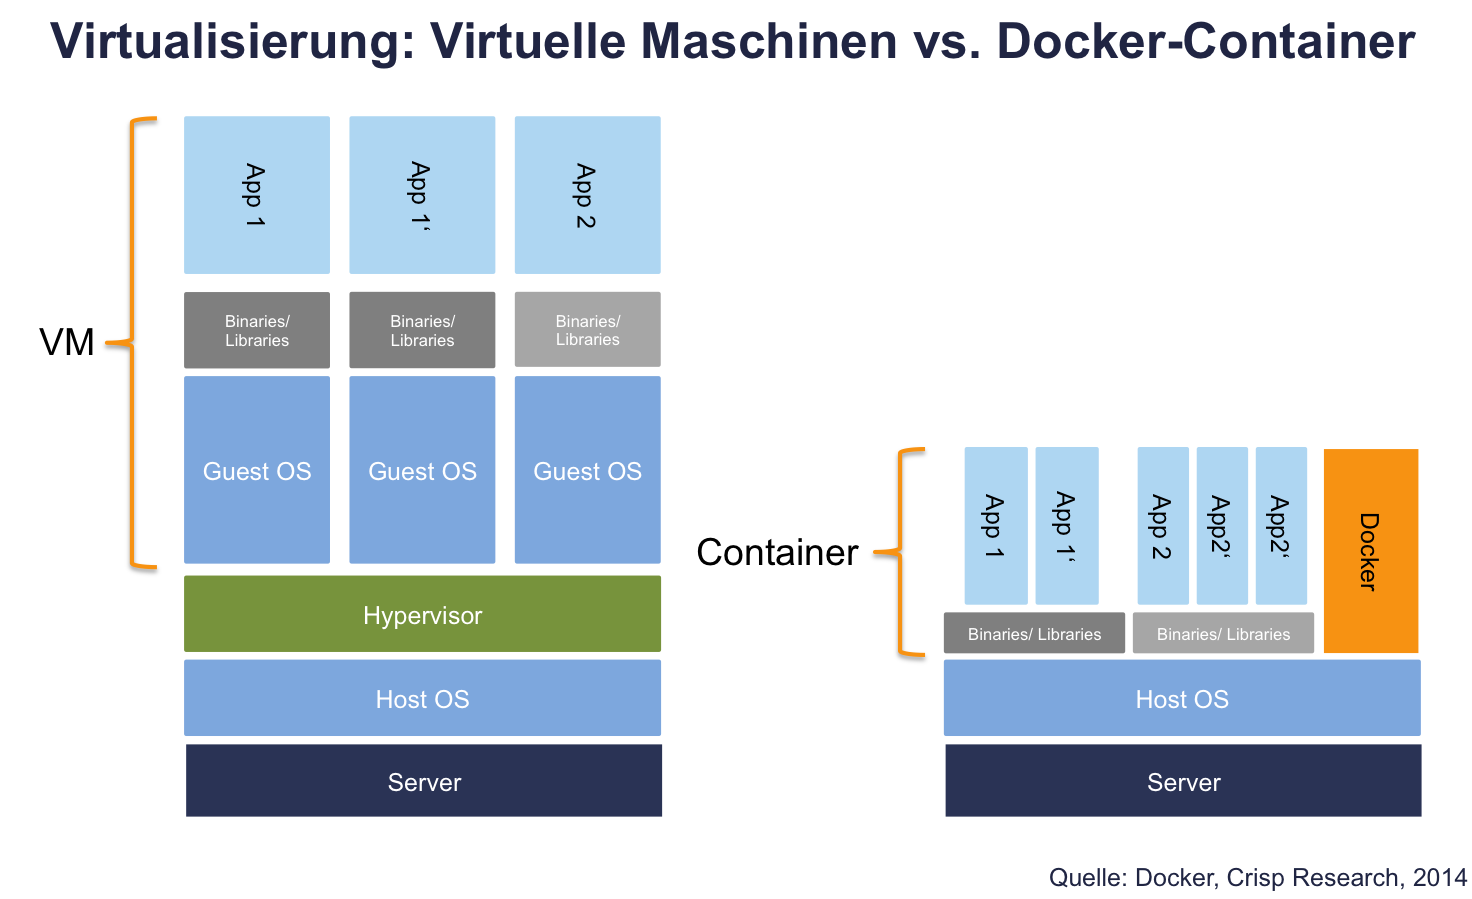
\includegraphics[width=1\textwidth]{containerundvm.png}
	\end{center}
	\caption[Vergleich Container und VM]{Vergleich Container und VM \footnotemark}
	\label{fig:VergleichContainerVM}
\end{figure}
\quellefoot{https://images.computerwoche.de/bdb/2668601/738x415_f5f5f5.jpg}
\newpage



\input{Inhalt/Funktionalität}
% !TEX root = ../Ausarbeitung.tex
\section{Containertechnologien} 
\label{sec:Containertechnologien}

In der Geschichte der Containertechnologie traten verschiedene Implementierungsformen auf.
Hierbei waren die ersten Umsetzungen noch sehr einfach aufgebaut und wurden mit den Anforderungen an die Containerdienste immer komplexer.
Im Folgenden findet sich eine Übersicht über die wichtigsten Technologien der Containerisierung.

\begin{figure}[H]
	\begin{center}
		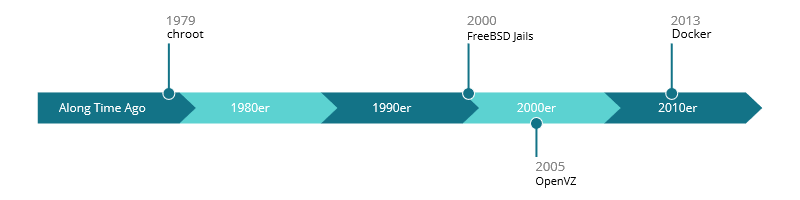
\includegraphics[width=1\textwidth]{ZeitContainer.png}
	\end{center}
	\caption[Containertechnologie im Laufe der Zeit]{Containertechnologie im Laufe der Zeit}
	\label{fig:CTZeit}
\end{figure}


\subsection*{chroot}
\label{sec:chroot}

Chroot ist ein Befehl, der schon früh in Unix-Systemen eingebaut wurde.
Er ermöglicht es einem Prozess, ein anderes Rootverzeichnis zu geben.
Wird in einem Programm \code{chroot()} aufgerufen, wechselt es das Verzeichnis und kann nicht auf Dateien außerhalb der zugewiesenen Struktur zugreifen.
Diese Abschottung eines Prozess war nie als Sicherheitsfeature vorgesehen und wird hauptsächlich zur Virtualisierung eingesetzt.
Mit dem Befehl können einzelne Prozesse auf Dateiebene von anderen Anwendungen getrennt werden, weitere Sicherheitsmechanismen oder Isolierungen gibt es nicht.\cite{IEEE7830207,569694, MANPAGE01}
\newpage
\subsection*{OpenVZ}
\label{sec:OpenVZ}

\begin{wrapfigure}{l}{0.4\textwidth}
	\vspace{-40pt}
	\begin{center}
		
\includegraphics[width=0.3\textwidth]{openvz.png}
	\end{center}
	\vspace{-15pt}
	\caption[Logo OpenVZ]{ \footnotemark}
	\label{fig:openvz}
	\vspace{-30pt}
\end{wrapfigure}
\quellefoot{https://upload.wikimedia.org/wikipedia/commons/b/bb/OpenVZ-logo.png?download}

Im Jahr 2005 veröffentlichte die Firma SWsoft (später umbenannt zu Parallels) ihr Projekt OpenVZ unter der GNU GPL Lizenz. OpenVZ basierte auf der Idee der Container, ermöglicht es jedoch in jedem Container eine eigene Linux-Distribution auszuführen.
Die durch die Containerumgebung abgegrenzten Betriebssysteme, teilen sich dabei einen Kernel. Dadurch ist der Overhead von OpenVZ deutlich geringer als bei der klassischen Vollvirtualisierung eines Betriebssystems.
In den einzelnen Containern gibt es jeweils einen eigenen root-User und eine eigene Dateistruktur.
Sie können unabhängig voneinander gestarten und gestoppt werden.
Da sich die Betriebssysteme einen Kernel teilen, können auch die Gastsysteme nur Linux-Systeme sein.
Da viele der Änderungen von OpenVZ den Kernel von Linux betreffen, werden regelmäßig Änderungen von OpenVZ-Patches in den Kernel von Linux übernommen.\cite{OpenVzNews, IEEE4803091,OpenVzHist}


\subsection*{FreeBSD Jails}
\label{sec:jails}
Mit der Veröffentlicheung von FreeBSD 4.0 im Jahr 2000 war FreeBSD Jails das erste richtige System in der Containervirtualisierung.
Die FreeBSD Jails basieren auf dem Konzept von chroot. Auch hier wird das root-Verzeichnis eines Prozess geändert. Zusätzlich verbessert Jails das Konzept um einige Aspekte, so erhält jede Jail einen eigenen Hostnamen	und eine eigene IP-Adresse. Jede Jail hat auch ihre eigenen Benutzer, inklusive einem root-Benutzer. \cite{FreeBSDHB14} Durch diese Prozessisolation ergibt sich eine Art Containersystem. Da die Jails als eigener Prozess laufen, können sie unabhängig voneinander gestartet und gestoppt werden.  Jails wird gerne für den Einsatz in Netzwerkaufgaben eingesetzt, da die Performance sehr gut ist. Jails besitzt allerdings kein so großes Ökosystem wie Bespielsweise Docker oder OpenVZ. Daher wird es in der Containervirtualisierung von diesen Gegenspielern verdrängt.


\subsection*{\ac{LXC}}
\label{sec:LXC}
\begin{wrapfigure}{r}{0.4\textwidth}
	\vspace{-40pt}
	\begin{center}
		\includegraphics[width=0.3\textwidth]{LXC.png}
	\end{center}
	\vspace{-15pt}
	\caption[Logo \ac{LXC}]{ \footnotemark}
	\label{fig:LXC}
	\vspace{-30pt}
\end{wrapfigure}
\quellefoot{https://upload.wikimedia.org/wikipedia/commons/4/40/Linux_Containers_logo.png?download}
\ac{LXC} ist seit der erstmaligen Veröffentlichung 2008 ein offizielles Kernelfeature und in den meisten Distributionen von Linux enthalten. \ac{LXC} ist eine User Space-Schnittstelle für die erstellung von isolierten Umgebungen innerhalb eines Systems. Dies geschieht durch die Nutzung von Kernel namespace, Apparmor und SELinux-Profilen sowie chroots und cgroups. Diese Features standen schon vor \ac{LXC} zur Verfügung, jedoch vereinigte sie \ac{LXC} zu einer Schnittstelle für die Erzeugung von Containern. Zu Beginn der Entwicklung von \ac{LXC} war die Isolation der Container nicht so gut, sondern glich eher einer Abwandlung der chroot-Funktion. Mit der Zeit wurde die Abschottung jedoch immer besser und die \ac{LXC}-Container wurden zu richtigen virtualisierten Umgebungen. Dies geschah unter anderem dadurch, dass ab Version 1.0 die einzelnen Container als unpriviliegierte Benutzter ausgeführt werden können. Zuvor war dies nicht möglich und eine Abgrenzung der Container nur bedingt gegeben. \ac{LXC} ist eine Technologie, die von vielen weiteren Projekten eingesetzt wird, unter anderen auch Proxmox oder Docker (bis Version 1.1)\cite{IEEE7036275, IEEE7185212, IEEE7571957,IEEE7929714,LXCHomepage}


\subsection*{LXD}
\label{sec:lxd}

Um die Verwendung von \ac{LXC} zu vereinfachen wurde das Tool LXD entwickelt. Es besteht aus drei Elementen: Einem Deamon, der eine REST-API zur Verfügung stellt, einem Befehlszeilenclient sowie einem Open-Stack Nova Plugin. Die vom Deamon bereit gestellte Schnittstelle ermöglicht es, über das Netzwerk auf das Management der Container zuzugreifen. LXD ist somit eine Erweiterung, die eine Schnittstelle zu \ac{LXC}-Containern schafft. Über das Nova Plugin können die einzelnen LXD-Maschinen als Rechenknoten verwendet werden. \cite{LXDHomepage}

\subsection*{Solaris Container}
\label{sec:solariscontainer}

Im Jahr 2004 veröffentlichte Oracle im Build 51 von Solaris 10 zum ersten Mal ein Feature mit dem Namen Solaris Containers. Solaris Container stellt eine Technologie dar, mit der auf x86 und SPARC-Systemen Betriebssystemlevelvirtualisierung durchgeführt werden kann. Später zusammengelegt zu Solaris Zones, bestanden die beiden Technologien Solaris Containers und Solaris Zones parallel zueinander. Dabei war Zones eine klassische Virtualisierungsplatform mit Hypervisor und Containers eine Containertechnologie, die analog zu chroot funktionierte. Mit der Zusammenlegung von Containers und Zones zum neuen Zones wurde daraus eine Containerumgebung, in der die Container sicher voneinander und dem Host getrennt sind und von einem Resourcenmanagement kontrolliert werden.\cite{OracleZonesIntro,OracleZonesOver}
	

%\subsection{Windows Containers}
%s\label{sec:WindowsContainers}



\subsection*{Docker}
\label{sec:Docker}


dotCloud veröffentlichte am März 2013 das Projekt mit dem Namen Docker, dieses Projekt stellte Solomon Hykes auf der PyCon 2013 zum ersten Mal der Öffentlichkeit vor. \cite{dockeryout1} Ein paar Monate Später kündigte dotCloud Inc. an, den Firmennamen zu Docker Inc. zu ändern und sich hauptsächlich der Entwicklung des Docker Ökosystems zu widmen.\cite{dockerblog} Die Firma Docker Inc. (im Folgenden "`Docker Inc."' oder "`Hersteller"') hat bis zum heutigen Tag das Projekt Docker (Im Folgenden "`Docker"') weiterentwickelt und das Ökosystem darum ausgebaut. So wurde unter Anderen der DockerHub eingerichtet, eine Plattform um Images zu teilen und auszutauschen.\cite{dockermanual}

Zu Beginn war Docker lediglich eine Werkzeugsammlung, um \ac{LXC}-Container zu verwalten, jedoch baute Docker Inc. diese Sammlung immer weiter aus und erweiterte das System um Funktionen, die vom unterliegenden Linux-Betriebssystem nicht gegeben waren. Mit der Version 0.9 veröffentlichte Docker Inc. den neuen Treiber libcontainer und nutzte ihn von dort an als native Umgebung für Docker-Container. \cite{dockerblog2} Zu Beginn unterstützte Docker lediglich Linux-Container und nutzte dazu unter Windows eine virtuelle Maschine (Windows 7 \& 8) oder das Linux-Subsystem (Windows 10). Ab der Version 17.11 von Docker für Windows und dem Windows 10 Fall Creators Update konnten erstmals Windows Containers genutzt werden. \cite{dockerblogwin} Auch entwickelte Docker Inc. weitere Zwischebenen, um sich von \ac{LXC} zu lösen und die Umgebung in Module zu teilen. So entstand containerd, ein Container-Deamon, mit dem die Docker Engine kommuniziert. Dieser Deamon wiederum kann mit einem OCI-konformen Container-Tool umgehen und über dieses Container starten. Ein solches Tool ist das eigene runC. Auf diese Art können Docker-Container auch durch andere Orchestrierungstools wie Kubernetes oder Swarm verwaltet werden (\Vgl \Abschnitt{Cluster}).\cite{Buch}

Zum heutigen Zeitpunkt ist Docker die führende Containerumgebung (\Vgl \Abbildung{Stats2}), daher ist die Funktion derselben im Folgenden anhand eines Beispielcontainers aufgezeigt:

In diesem Beispiel soll innerhalb eines Docker-Containers ein python-Skript ausgeführt werden. Zu Beginn eines jeden Containers steht ein Image. Auf diesem schreibgeschützten Image basiert später eine schreibbare Container-Instanz. Ein Image enthält alle benötigten Teile des OS abgesehen vom Kernel, denn dieser wird bereits durch den Host zur Verfügung gestellt. Zusätzlich gehören auch benötigte Anwendungen zu einem Image. Auf diesem schreibgeschützten Teil wird dann ein schreibbarer Layer aufgebaut, wenn von dem Image eine Container-Instanz abgeleitet wird. Wird die Container-Instanz beendet, sind alle Änderung innerhalb des schreibbaren Layer verloren. Um die Änderungen zu sichern kann ein sogenannter Snapshot angelegt werden, der dem Image ein weiteres read-only-Layer hinzufügt. Die Anzahl der Layer ist, je nach Docker-Version auf 127 beschränkt. \cite{Buch, dockermanual} Zum Beispiel könnte ein Image für den Beispielcontainer wie folgt aussehen:

\begin{figure}[h]
    \vspace{-10pt}
    \begin{center}
        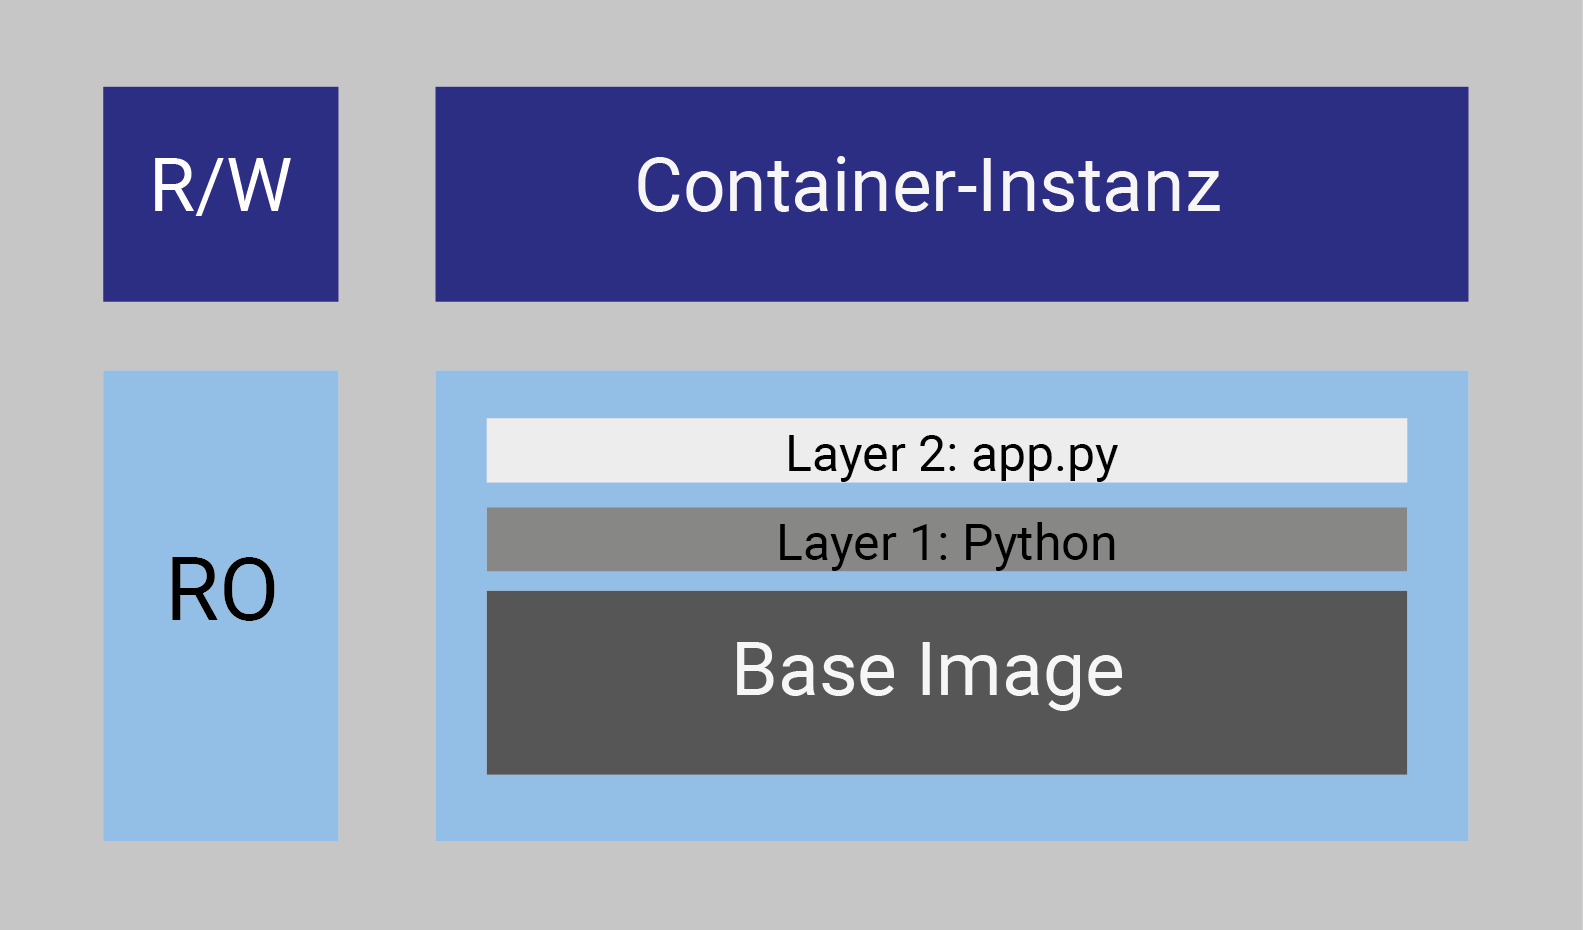
\includegraphics[width=0.6\textwidth]{DockerImage.png}
    \end{center}
    \caption[Image des Beispielcontainer ]{Image des Beispielcontainer}
    \label{fig:docker1}
    \vspace{-10pt}
    \end{figure}

Als Basis dient ein Image, in dem Alpine Linux installiert ist und darauf python. Zu diesen Layern wollen wir noch das python-Skript hinzufügen. Dies ist dann der schreibgeschützte Teil, von dem der Container abgeleitet wird. In dieser Container-Instanz legt das python-Skript dann Dateien an und schreibt in diese. Wird der Container dann beendet, werden alle angelegten Dateien verworfen.\\
Dieses Image kann in einem Dockerfile beschrieben werden. Dies sieht für diesen Fall wie folgt aus:

\begin{lstlisting}[language=docker,label={code:dockerfile}]
    FROM python:3
    
    WORKDIR /usr/src/app
    
    COPY ./app.py ./app.py
    
    CMD ["python", "./app.py"]
\end{lstlisting}

In dem Dockerfile wird zuerst definiert, dass das Image auf vorhanden dem python-Image aufbauen soll. Dieses wiederum baut auf einem Alpine-Linux-Image auf. Daraufhin wird das aktuelle Arbeitsverzeichnis im Container geändert. Dann wird die im Arbeitsverzeichnis des Host abgelegte Datei "`app.py"' in das Arbeitsverzeichnis des Container übertragen und schließlich der Befehl definiert, der beim Starten des Container ausgeführt werden soll. Das Python-Skript legt ein Datei an und gibt deren Dateiname und Inhalt zur Konsole aus:
\begin{lstlisting}[language=python,label={code:pythonapp}]
#!/usr/bin/python3

print("Ausgabe zur Kommandozeile")
file=open("datei.txt", "a+")
print("Dateiname: ", file.name)
file.write("Eine neue Zeile")
file.close()
print(open("datei.txt","r").read())
\end{lstlisting}
Nun kann mit dem Befehl \code{docker build} das Image erstellt werden. Dabei lädt Docker zunächst das Image von python aus dem oben genanten Docker-Hub herunter und legt darauf das Layer mit dem python-Skript:

\begin{lstlisting}[language=bash,label={code:dockerbuild}]
user@dockerpc:~$ docker build -t pythontest .
Sending build context to Docker daemon 311.4MB
Step 1/4 : FROM python:3
 ---> 638817465c7d
Step 2/4 : WORKDIR /usr/src/app
---> 8d3ab23442c9
Step 3/4 : COPY ./app.py ./app.py
---> 2b0882cadee4
Step 4/4 :  CMD ["python", "./app.py"]
---> 5a8a392a0856
Successfully built 5a8a392a0856
Successfully tagged pythontest:latest
\end{lstlisting}

Nun liegt das Image bereit und es kann ein Container davon abgeleitet werden. Dazu reicht nur der einfache Befehl \code{docker run} um den Container zu starten:

\begin{lstlisting}[language=bash,label={code:dockerbuild}]
user@dockerpc:~$ docker run pythontest
Ausgabe zur Kommandozeile
Dateiname: datei.txt
Eine neue Zeile
\end{lstlisting}

Hier wird nun das Python-Skript in dem Container ausgeführt und der Container daraufhin beendet und somit auch die beschriebene Datei gelöscht. Wird der Container erneut ausgeführt, so wird eine neue Datei erstellt:

\begin{lstlisting}[language=bash,label={code:dockerbuild}]
user@dockerpc:~$ docker run pythontest
Ausgabe zur Kommandozeile
Dateiname: datei.txt
Eine neue Zeile

user@dockerpc:~$ docker run pythontest
Ausgabe zur Kommandozeile
Dateiname: datei.txt
Eine neue Zeile
\end{lstlisting}

Die Layer, aus denen Docker die verschiedenen Images aufbaut wurden von Docker Inc. zu dem ursprünglichen \ac{LXC}-Container hinzugefügt und später zum hauseigenen libcontainer übernommen. Durch diese Layer ist es einfacher Ressource zu teilen. Wenn mehrere Images auf Pyhton oder Alpine-Linux aufbauen sollen, so müssen diese beiden Ressourcen nicht mehrfach heruntergeladen werden, sondern können jedem Image zur Verfügung gestellt werden. Dies ist einer der Gründe, warum Docker nach der Veröffentlichung eine große Popularität erreichte und heute die führende Containertechnologie ist.\cite{dockermilestones}



\subsection*{rkt}
\label{sec:rkt}

\begin{wrapfigure}{l}{0.4\textwidth}
	\vspace{-40pt}
	\begin{center}
		
\includegraphics[width=0.3\textwidth]{rkt.png}
	\end{center}
	\vspace{-15pt}
	\caption[Logo rkt]{ \footnotemark}
	\label{fig:rkt}
	\vspace{-30pt}
\end{wrapfigure}
\quellefoot{https://github.com/rkt/rkt/raw/master/logos/rkt-horizontal-color.png}


rkt (Ausprache wie "rocket") ist eine Containerengine, die sich als Alternative zu Docker etabliert und von CoreOS veröffentlicht wurde und weiterentwickelt wird. Das Projekt ist ein Open-Source-Projekt und unter der Apache License 2.0 veröffentlicht.\cite{RepoRkt} Unter rkt werden viele Grundgedanken von UNIX umgesetzt, so liegen alle Container als Dateien vor, die einfach verwaltet werden können. Auch legt rkt einen großen Wert auf Sicherheit und setzt dazu verschiedene Techniken ein, die inzwischen von den meisten Konkurennten übernommen wurden. So kann rkt für jeden Container entscheiden, ob dieser auf Basis von KVM oder einer Virtual Machine isoliert wird und führt alle Prozesse, auch den Download von Images, als nicht priviligierter Benutzer aus. In rkt wird die kleinste Einheit ein "pod" genannt. Sie kann aus einem oder mehrerm Containeren bestehen, die sich Ressourcen teilen. So passt das Konzept von  rkt direkt zu den Konzepten von  Cluster-Managern. Auch besitzt rkt keinen zentralen Service, der alle Container überwacht, sondern arbeitet direkt mit dem Systemeigenen systemd zusammen, um die Container zu verwalten. Somit lässt sich rkt auch direkt mit Kubernetes verknüpfen, für das der Herausgeber von rkt, CoreOS, die kommerzielle Implementierung Tectonic entwickelt. rkt unterstützt auch die Konvertierung von Docker-Containern zu rkt-Pods.\cite{HomepageRkt,ixrkt}


% !TEX root = ../Ausarbeitung.tex
\section{Container und Softwareentwicklung} 
\label{sec:Softwareentwicklung}

Der Einsatz von Containern erleichtert die Entwicklung von Software in vielerlei Hinsicht. So müssen Entwickler ihre Applikationen für verschiedene Plattformen nicht grundlegend verschieden entwerfen und die Programmiersprache kann meist frei gewählt werden. 
Ob für Windows, Linux, MacOS, Cloud-Plattformen oder andere, der Fokus der Entwicklung kann deutlich stärker auf die Funktionalitäten der Applikation gerichtet werden, wenn die Eigenheiten der Ziel-Plattform in den Hintergrund rücken. Das macht den gesamten Entwicklungsprozess einfacher und somit effizienter.
Mithilfe der Abstraktion durch Container vermeidet man Inkompatibilitätsprobleme auf den Host-Geräten und auch die Entwicklung sowie Softwaretests gestalten sich dadurch leichter, schneller und effizienter, denn alle für die Applikation wichtigen Daten, Tools und Systembibliotheken sind im Container vorhanden.
\cite{11517836120160501}

Entwickler können davon ausgehen, dass ihre Applikation auf verschiedenen Systemen funktionieren wird und können sie immer unter konsistenten Bedingungen testen, egal wie später die Umgebung aussehen mag. Dies erhöht die Zuverlässigkeit enorm. Man ist nicht länger Abhängig von der Verfügbarkeit von identischen Entwicklungs- und Testsystemen und der Entwickler kann auf seinem eigenen Rechner auch schnelleres Feedback erhalten, wenn er den Container lokal ausführt und debuggt.

Auch ermöglichen Container die Verwendung von Microservices. Sonst als monolithische Applikation entworfene Software kann von Entwicklern unabhängig in mehreren Teilen erstellt werden, was die Agilität deutlich fördert.
Außerdem ist das Software Deployment sehr simpel, da es nur gilt, ein Container Image zu erzeugen und zu verteilen. Dies kann auch über Container-Orchestration-Tools wie Kubernetes nach dem Prinzip von Continous Delivery automatisiert werden. Die Ausführung läuft auf jedem System dann jedes Mal gleich ab.
%Jonas PDF\cite{}

Dementsprechend benötigt man auch für Weiterentwicklung und Wartung der Applikationen weniger Zeit und Personal als wenn man für jedes System eigene Entwickler mit Fachkenntnissen bräuchte.
Bei Veränderungen an der Hardware, kurzfristigem Wechsel, Neuanschaffungen aber auch bei Upgrades des Betriebssystems hat eine Firma keine größeren Schwierigkeiten durch Inkompatibilitäten zu befürchten. Somit ist sie auch freier in der Wahl ihrer Geräte.

Auch das sogenannte Monitoring, die laufende Überwachung der Systeme, über Schnittstellen (APIs) ist mit Containern kein Problem. Logs können von jeder Applikation erstellt, dann einfach gesammelt und in ein Management-System übertragen werden. Die Erkennung und Eingrenzung von Fehlerquellen beschleunigt sich dadurch, dass die Applikation im Container gekapselt ist und keine weiteren Programme oder Betriebssystemteile die Fehlersuche erschweren. Auch können die Container-Applikationen einfach mit ihrem vordefinierten Idealzustand neugestartet werden, sobald ein Problem erkannt wird.
Diese Vereinfachung durch Abstraktion hilft dann nicht nur dem Entwickler, sondern trägt zur Zufriedenheit der Nutzer bei. 

Besonders wenn es darum geht, neue Applikationen zu entwerfen, deren Zielplattformen noch nicht endgültig festgelegt sind, oder bei einem Umzug in die Cloud. Gerade bei Cloud-Diensten sind Container unter anderem wegen ihres geringeren Ressourcen-Umfangs beliebt.
\cite{12771285120180201}

"Container eignen sich optimal für dienstbasierte Architekturen. Im Gegensatz zu monolithischen Architekturen, bei denen alle Teile einer Anwendung miteinander verknüpft sind […], werden diese Komponenten bei einer dienstbasierten Architektur getrennt. Durch eine Trennung und Arbeitsteilung werden Ihre Dienste auch dann weiter ausgeführt, wenn andere fehlschlagen. Damit bleibt Ihre gesamte Anwendung zuverlässiger."\footnote{\url{https://cloud.google.com/containers/}}

Tools, die sich speziell um das Ressourcen-Management kümmern, sind in vielen Containern mit inbegriffen, sodass beispielsweise der zur Verfügung stehende Speicher sinnvoll begrenzt werden kann, um Out-of-memory-Abstürzen vorzubeugen. 
Das schont die Server, auf denen die Applikationen laufen, und reduziert den Hardware-Bedarf und die Kosten, wenn weniger virtuelle Maschinen mit eigenem vollwertigen Betriebssystem aufgesetzt werden müssen.
\cite{11517836120160501}
% !TEX root = ../Ausarbeitung.tex
\section{Cluster}
\label{sec:Cluster}
Wie in \Abschnitt{Einleitung} genannt, wurden in der Vergangenheit dedizierte Server für jeweils einen Service genutzt.
Dies hatte den Nachteil einer geringen Serverauslastung sowie bei nicht reundanten Servern die Gefahr eines Totalausfalls eines Services.
Applikationen ließen sich nicht ohne weiteres von einem Server auf einen anderen umziehen, da sie tief in das Hostsystem integriert waren.

Cluster Manager verbinden mehrere Maschinen zu einer Einheit. Während Lösungen wie Apache Mesos eine Abstraktion der Hardware vornehmen, basieren Kubernetes und Docker Swarm auf der Container-Architektur.
Diese Cluster Manager übernehmen die Verwaltung der Container sowie ihre Zuordnung zu den jeweiligen Maschinen.

Clustering sorgt für eine verbesserte Redundanz und erhöht somit die Ausfallsicherheit.
Außerdem lässt sich so eine bessere Ressourcen-Allokation vornehmen.

Thema aktueller Forschungsarbeiten ist die Verbesserung des Sheduling, um die Ressourcennutzung zu optimieren.\cite{Liu2018}


% !TEX root = ../Ausarbeitung.tex
\section{Risiken der Containertechnologie}
\label{sec:Risiken der Containertechnologie}
% Einleitung mit Fragestellung
Die Containertechnologie erobert in den letzten Jahren mehr und mehr die Rechenzentren. Doch welche Risiken verbergen sich dahinter und wie kann man sich schützen?

% Multiplizierung von Sicherheitslücken
Durch die hohe Anzahl an Container pro Server ist das Risiko bei einer Sicherheitslücke deutlich höher, da sich diese dann in beispielsweise 80 Containern, anstatt in vier virtuellen Maschinen oder einem dedizierten Server ausnutzen lässt.\cite{Risiken}

% Risiko infizierter Images
Um sich den Aufwand für die Konfiguration der Images zu sparen (diese kann sehr aufwendig sein), verwenden viele Administratoren vorgefertigte Container aus einem Respository.
Dabei muss dem Ersteller vertraut werden, dass das Image keinen Schadcode oder Hintertüren enthält, da der Aufwand für eine genaue Prüfung des Container-Inhalts sehr aufwendig wäre.
Im Juni 2018 hatte die Sicherheitsfirma Kromtech berichtet, dass über das Repository Docker Hub mehrere Images über ein Jahr lang verfügbar waren, die Schadcode zum Minen von Kryptowährungen enthielten.
Diese wurden insgesamt fünf Millionen mal installiert, bevor die Betreiber von Docker Hub reagierten und diese entfernten.
\cite{kromtech}
Die betroffenen Administratoren hätten das Risiko minimieren können, indem sie nur über das offizielle Docker Repository die Container bezogen hätten.
Dort werden Images vor ihrer Veröffentlichung geprüft.
\cite{DockerHubOfficial}
Ein Angreifer müsste zur Verteilung eines infizierten Images den Schadcode verstecken, sodass er bei der Prüfung nicht sichtbar wird. Dies stellt eine wesentlich höhere Hürde dar.

% Schnittstellen zum Kernel
Werden Applikationen in Containern richtig verpackt, so sind die einzigen Abhängigkeiten nach außen hin die Systemaufrufe des Betriebssystems.
Dies verbessert die Portabilität der Anwendungen ungemein, allerdings sind auch Systemaufrufe wie z.B. Socket-Schnittstellen sowie hardwarespezifische Systemaufrufe nicht auf allen Systemen einheitlich, wodurch die Portabilität eingeschränkt wird.
Die Open Container Initivative der Linux Foundation arbeitet neben einem Standard für Container Formate auch an einem Standard für Container Runtimes.
Dieser könnte helfen, die Schnittstelle zwischen Container und Betriebssystem besser festzulegen.

% Probleme mit Hardware
Container können nicht gegen Einflüsse schützen, die nicht vom Betriebssystem verwaltet werden. Hierzu sind virtuelle Maschinen als zusätzliche Sicherheitsschicht notwendig.\cite{11517836120160501}

% Prozessorprobleme
Nicht zuletzt haben die Sicherheitslücken Meltdown (\cite{DBLP:journals/corr/abs-1801-01207}) und Spectre (\cite{DBLP:journals/corr/abs-1801-01203}) gezeigt, dass über Sicherheitslücken in Prozessoren containerübergreifende Angriffe auf Applikationen möglich sind. Hiergegen schützten virtuelle Maschinen allerdings ebenfalls nicht.  

% !TEX root = ../Ausarbeitung.tex
\newpage
\section{Aktuelle Lage}
\label{sec:AktuelleLage}
\Abbildung{Stats1} zeigt, dass trotz einiger Risiken der Container Technologie Unternehmen weltweit immer mehr Geld in die Containerisierung ihres Unternehmens investieren. Laut einer Umfrage, welche auf der DockerCon durchgeführt wurde, investierten 32\% der Unternehmen mindestens 500.000\$ jährlich, um die Containerisierung in ihrer Organisation voranzutreiben. \citep{Investments}
\begin{figure}[H]
	\begin{center}
		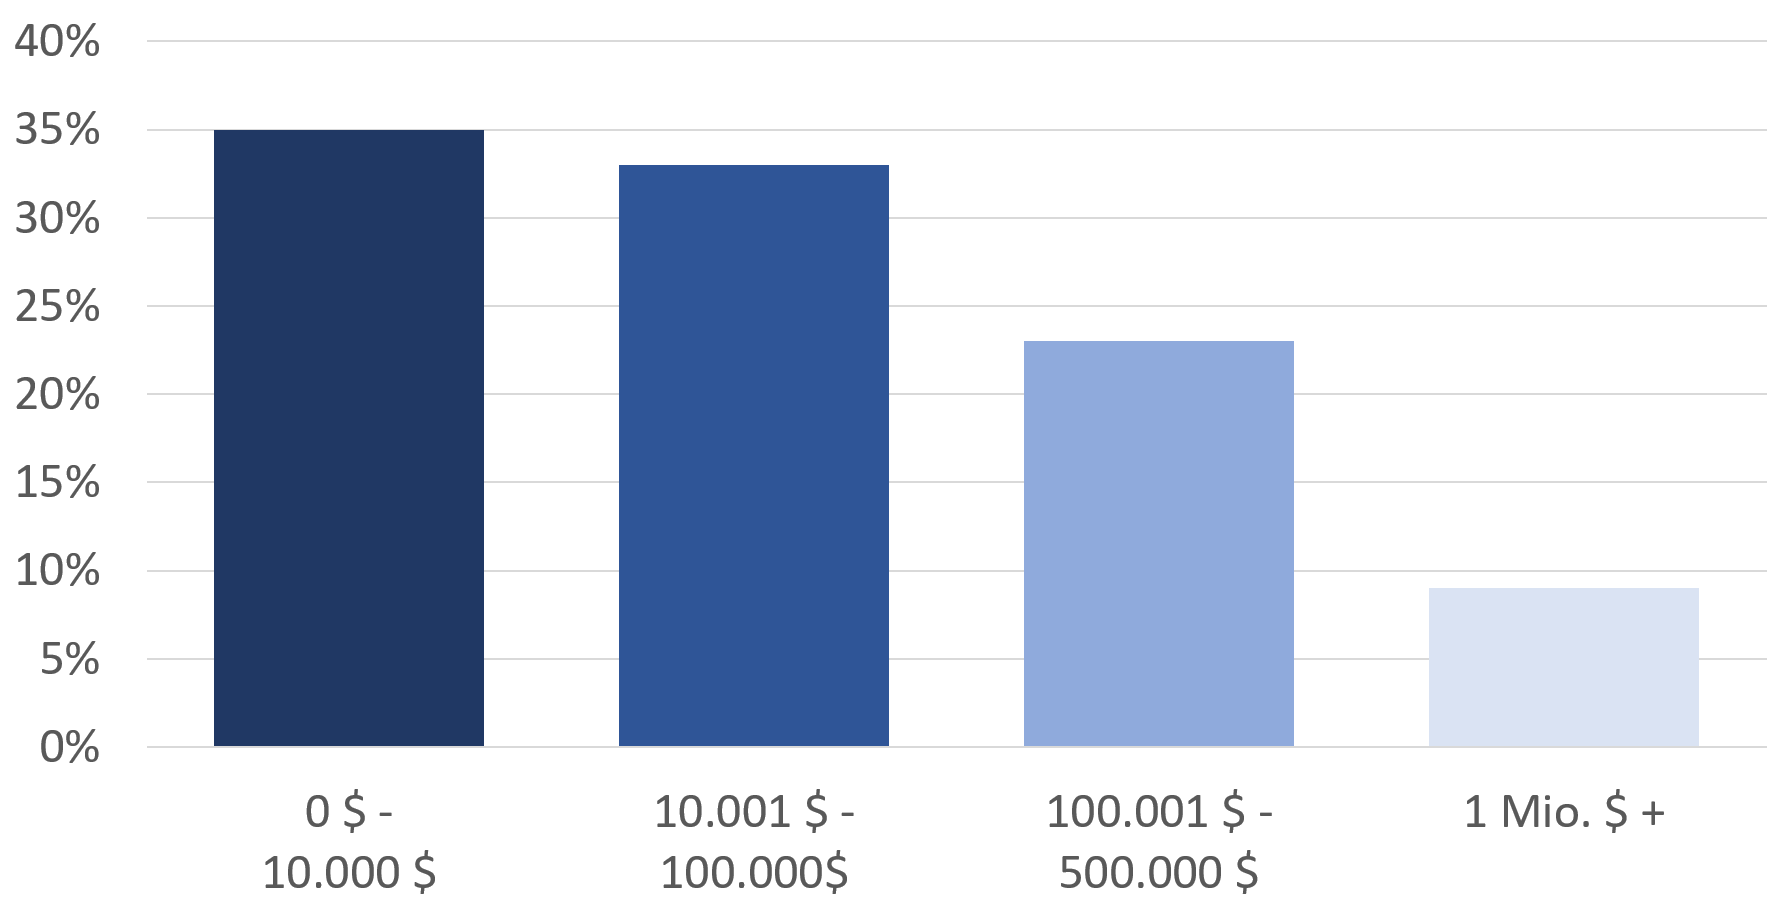
\includegraphics[width=0.8\textwidth]{ContainerInv.png}
	\end{center}
	\caption[Investitionen in die Containerisierung]{Investitionen in die Containerisierung}
	\label{fig:Stats1}
\end{figure}

\newpage
Aus \Abbildung{Stats2} ist zu entnehmen, dass 83\% der produktiv eingesetzten Container von Docker stammen. An zweiter Stelle der meist verwendeten Container findet sich CoreOS, welches von der Firma Red Hat übernommen wurde. Mesos Containerizer und \ac{LXC} machen zusammen nur 5\% aller eingesetzten Container aus. \citep{stats}
\begin{figure}[H]
	\begin{center}
		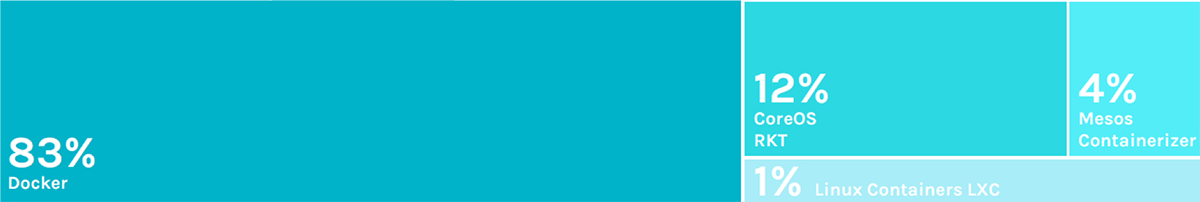
\includegraphics[width=1\textwidth]{DockerProzent.png}
	\end{center}
	\caption[Benutzung von Containertechnologien]{Benutzung von Containertechnologien \footnotemark}
	\label{fig:Stats2}
\end{figure}
\quellefoot{https://www.dailyhostnews.com/wp-content/uploads/2018/05/d2.png}
Laut eines Berichts der Container-Monitoring-Firma Sysdig stieg die Anzahl der durchschnittlich verwendeten Container pro Host 2018 um 50\% im Vergleich zum Vorjahr. Das entspricht nun etwa 15 Containern. Laut des Berichts ist 154 die höchste Anzahl von Containern, die bisher gleichzeitig auf einer Maschine laufen. \citep{stats} \Abbildung{Stats3} stellt dies grafisch dar.
\begin{figure}[H]
	\begin{center}
		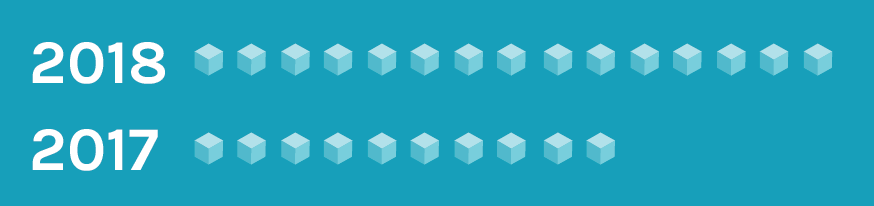
\includegraphics[width=0.8\textwidth]{ContainerHost.png}
	\end{center}
	\caption[Container je Maschine]{Container je Maschine \footnotemark}
	\label{fig:Stats3}
\end{figure}
\quellefoot{https://www.dailyhostnews.com/wp-content/uploads/2018/05/d1.png}
\newpage
Kubernetes sei die meist genutzte Plattform, um Container zu orchestrieren und wird von Software-Unternehmen wie Microsoft und IBM verwendet. Das beliebteste Tool, um Container-Cluster für große Firmen auszurollen, sei jedoch Mesos Containerizer. \citep{stats} Die genaue Verteilung ist \Abbildung{Stats4} zu entnehmen.
\begin{figure}[H]
	\begin{center}
		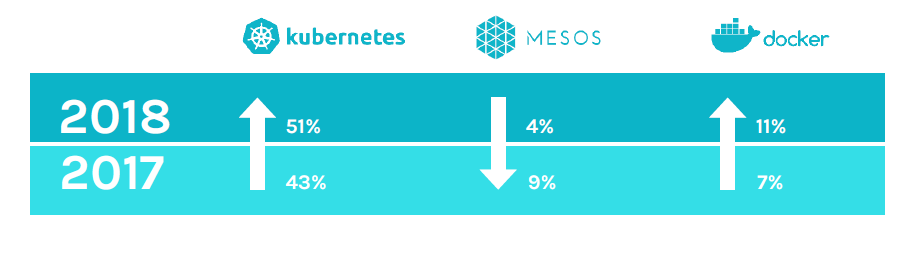
\includegraphics[width=0.8\textwidth]{Manager.png}
	\end{center}
	\caption[Cluster-Manager]{Cluster-Manager \footnotemark}
	\label{fig:Stats4}
\end{figure}
\quellefoot{https://www.dailyhostnews.com/wp-content/uploads/2018/05/d4.png}


% !TEX root = ../Ausarbeitung.tex
\section{Fazit und Ausblick} 
\label{sec:Fazit}







% Verzeichnisse
\clearpage
\listoffigures
%\cleardoublepage

\listoftables
%\cleardoublepage

\lstlistoflistings
%\cleardoublepage

\newcommand{\abkvz}{Abkürzungsverzeichnis}
\renewcommand{\nomname}{\abkvz}
\section*{\abkvz}
\markboth{\abkvz}{\abkvz}
\addcontentsline{toc}{section}{\abkvz}
% !TEX root = Projektdokumentation.tex

% Es werden nur die Abkürzungen aufgelistet, die mit \ac definiert und auch benutzt wurden. 
%
% \acro{VERSIS}{Versicherungsinformationssystem\acroextra{ (Bestandsführungssystem)}}
% Ergibt in der Liste: VERSIS Versicherungsinformationssystem (Bestandsführungssystem)
% Im Text aber: \ac{VERSIS} -> Versicherungsinformationssystem (VERSIS)

% Hinweis: allgemein bekannte Abkürzungen wie z.B. bzw. u.a. müssen nicht ins Abkürzungsverzeichnis aufgenommen werden
% Hinweis: allgemein bekannte IT-Begriffe wie Datenbank oder Programmiersprache müssen nicht erläutert werden,
%          aber ggfs. Fachbegriffe aus der Domäne des Prüflings (z.B. Versicherung)

% Die Option (in den eckigen Klammern) enthält das längste Label oder
% einen Platzhalter der die Breite der linken Spalte bestimmt.
\begin{acronym}[WWWWW]
	\acro{API}{Application Programming Interface}
	\acro{CSS}{Cascading Style Sheets}
	\acro{CSV}{Comma Separated Value}
	\acro{CI}{Continous Integration}
	\acro{EPK}{Ereignisgesteuerte Prozesskette}
	\acro{ERM}{En\-ti\-ty-Re\-la\-tion\-ship-Mo\-dell}
	\acro{HTML}{Hypertext Markup Language}\acused{HTML}
	\acro{LDAP}{Lightweight Directory Access Protocol}
    \acro{SASS}{Syntactically Awesome Stylesheets}
	\acro{IDE}{Integrated Development Environment}
	\acro{SDK}{Software Development Kit}
	\acro{SaSS}{Software as a Service}
	\acro{SQL}{Structured Query Language}
	\acro{SVN}{Subversion}
	\acro{UML}{Unified Modeling Language}
	\acro{XML}{Extensible Markup Language}
	\acro{FVSS}{Ferdinand-von-Steinbeis-Schule}
    \acro{UI}{Benutzeroberfläche (engl.: "`User Interface"')}
    \acro{SCSS}{Sassy CSS}
    \acro{VCS}{Version Control System}
    \acro{MVC}{Model-View-Controller}
    \acro{CI}{Kontinuierliche Integration (engl.: "Continuous Integration")}
    \acro{DI}{Dependency Injection}
    \acro{DRY}{Wiederhole dich nicht (engl.: Don't repeat yourself)}
\end{acronym}


% Literatur ------------------------------------------------------------------

\renewcommand{\refname}{Literaturverzeichnis}
\bibliography{Bibliographie}
\bibliographystyle{Allgemein/natdin} % DIN-Stil des Literaturverzeichnisses
%\bibliographystyle{alphadin}
%% !TEX root = Projektdokumentation.tex
\clearpage
\addsec{Eidesstattliche Erklärung}

% Hinweis: die eidesstattliche Erklärung ist ggfs. an die Richtlinie der IHK anzupassen

Ich, \autorName, versichere hiermit, dass ich meine \textbf{\betreff} mit dem
Thema
\begin{quote}
\textit{\kompletterTitel}
\end{quote}
selbständig verfasst und keine anderen als die angegebenen Quellen und Hilfsmittel benutzt habe,
wobei ich alle wörtlichen und sinngemäßen Zitate als solche gekennzeichnet habe. Die Arbeit
wurde bisher keiner anderen Prüfungsbehörde vorgelegt und auch nicht veröffentlicht.\\[6ex]

\abgabeOrt, den \abgabeTermin


\rule[-0.2cm]{5.5cm}{0.5pt}

\textsc{\autorName}
 % Eidesstattliche Erklärung nur wenn von nöten drucken

% Anhang ---------------------------------------------------------------------
\clearpage
\appendix
\pagenumbering{Roman}
% !TEX root = Ausarbeitung.tex
\section{Anhang}
\label{sec:anhang}
\subsection{Begründung der ausgewählten Literatur}
\label{app:BegruendungLiteratur}
% Container sind sehr neu
Zur Verfügung stand lediglich sehr aktuelle Literatur, da die Containervirtualisierung erst seit Erscheinen von Docker im Jahr 2013 in der IT-Branche an Bedeutung gewonnen hat. Daher sind auch viele der hier betrachteten Werkzeuge erst in den vergangen Jahren entwickelt worden.

% Kurzer Zeitraum der Bearbeitung
In  Anbetracht des kurzen Zeitraumes, der den Autoren zur Verfügung stand, konnte keine Fernleihe durchgeführt werden.
Eine Vorbestellung der Literatur war daher ebenfalls nicht möglich.
Am ersten Tag der Bearbeitung des Artikels stand außerdem die Bibliothek aufgrund des Betriebsausflugs nicht zur Verfügung, weshalb auch nicht auf die physischen Medien zurückgegriffen werden konnte.
Deshalb hat sich die Bücher- bzw. Artikelauswahl auf die über die Hochschule verfügbaren digitalen Medien beschränkt.

% Dokumentationen
Die  Literaturauswahl umfasst außerdem Dokumentationen der gängisten Software zum Thema Container-Technologie.
Diese wurde zum Verständnis des Aufbaus und der Nutzung des jeweiligen Werkzeugs genutzt. 
Die Dokumentationen sind online bzw. zusammen mit dem jeweiligen Source Code verfügbar und werden von den Entwicklern zur  Verfügung gestellt. 
Daher handelt es sich bei den Dokumentationen um eine verlässliche Quelle über das jeweilige Werkzeug.


% Offizelle Homepage
Auf den offizellen Webseiten der verschiedenen Hersteller und Projekten werden von den Entwicklern oder Firmen offizelle Informationen publiziert oder auch oben genannte Dokumentationen veröffentlicht. Der Inhalt der Webseiten kann als verlässliche Quelle angesehen werden, da hier der Ersteller des Produkts direkt veröffentlicht.


% Blogs
Blog Einträge dienten den Autoren als Ideengeber für einen Teil des Inhalts der vorliegenden Arbeit.
Da diese am Puls der Zeit sind, zeigen sie aktuelle Trends und populäre Software zum Thema Container-Technologie auf.
Ein Blog wird nicht überprüft und stellt daher selbstverständlich keine zuverlässige Quelle dar.
Zur weiteren Recherche wurden aufgrund dessen wissenschaftlich verlässliche Quellen verwendet.




\end{document}
